\section{Results}\locallabel{sec:results}
In this section we describe the results of our analysis of the \sone{} and
\stwo{} data. In general we wanted to gain insight into the following
questions:

\begin{itemize}
\item How successful were students in creating a \sprogram{} that completed the
  assignment?
\item Did the changes we make after \sone{} improve student completion rates?
\item How pervasive were the challenges identified by education researchers via
  direct student observation?
\end{itemize}

To answer these questions we (Section~\localref{sub:by_class}) look at the
completion rate of students by class, (Section~\localref{sub:snapshots})
compare the difficulty of \sone{} and \stwo{} based on the number of snapshots
to completion, (Section~\localref{sub:approach}) analyze the approach students
used in solving the assignment, (Section~\localref{sub:race}) quantify the
number of students who may have experienced a race condition in Scratch, and
(Section~\localref{sub:dce}) quantify the number of students who may have
utilized the \dce{} approach when initially working on the assignment.


\subsection{Students by Class}
\locallabel{sub:by_class}

\begin{figure}[!t]
\centering
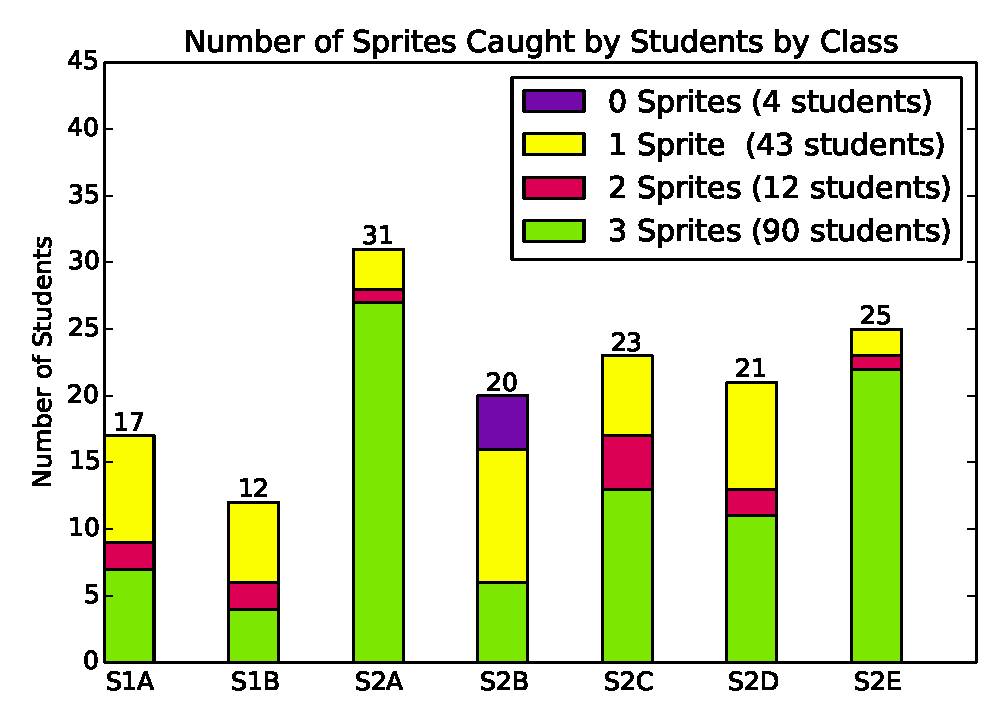
\includegraphics[width=5.25in]{graphs/by_class_students.eps}
\caption{Compares the maximum number of sprites \caught{} by student by
  class. A student is considered \com{} if any of their snapshots \catch{es}
  two or more sprites.}
\locallabel{fig:by_class_students}
\end{figure}

We analyzed data from seven of the ten classes listed in
Table~\localref{table:classes}: two for \sone{}, and five for \stwo{}. This
data include a total of 297 snapshots, twenty-nine students for \sone{}, and
638 snapshots, 120 students for \stwo{}. We have more data for \stwo{} due to
having more participating classes, all of which, contained more students for
whom we had consent.

Figure~\localref{fig:by_class_students} compares student completion of the
assignment for each class where the total height of each bar indicates the
number of students by class; this number is enumerated above each bar. The
different colored portions of each bar groups students by the maximum number of
sprites \caught{}. Green, pink, and yellow respectively indicate that all, two,
or only one of the three sprites were \caught{}. Purple indicates none of those
students' snapshots result in the \net{} \catch{ing} a sprite upon
execution. The four students in the \emph{0 Sprites} group are interesting
because the base-project provided to all students already \catch{es} one
sprite, the \zebra{}. Thus, these four students made changes resulting in
negative progress toward the goal. Also, it is noteworthy that of the 102
students who \caught{} at least two sprites, only twelve (11.8\%) did not
\catch{} the final sprite.

We determine the success of a snapshot by running it through a Hairball plugin
that emulates the \net{'s} movement according to the \net{} \emph{script}
beginning with the \netclicked{} block. A snapshot is considered \com{} if the
emulated movement of the \net{} results in intersection with any two or more
sprites corresponding to the \bear{}, \horse{}, and \zebra{}. In the event
intersection with the \snake{} occurs (only valid for \sone{}), the snapshot is
considered \incom{}. Of the 297 \sone{} snapshots, only one was \incom{} due to
intersection with the \snake{}. A student is considered \com{} if they have at
least one \com{} snapshot.

\subsection{Number of Snapshots to Completion}
\locallabel{sub:snapshots}

\begin{figure}[!t]
\centering 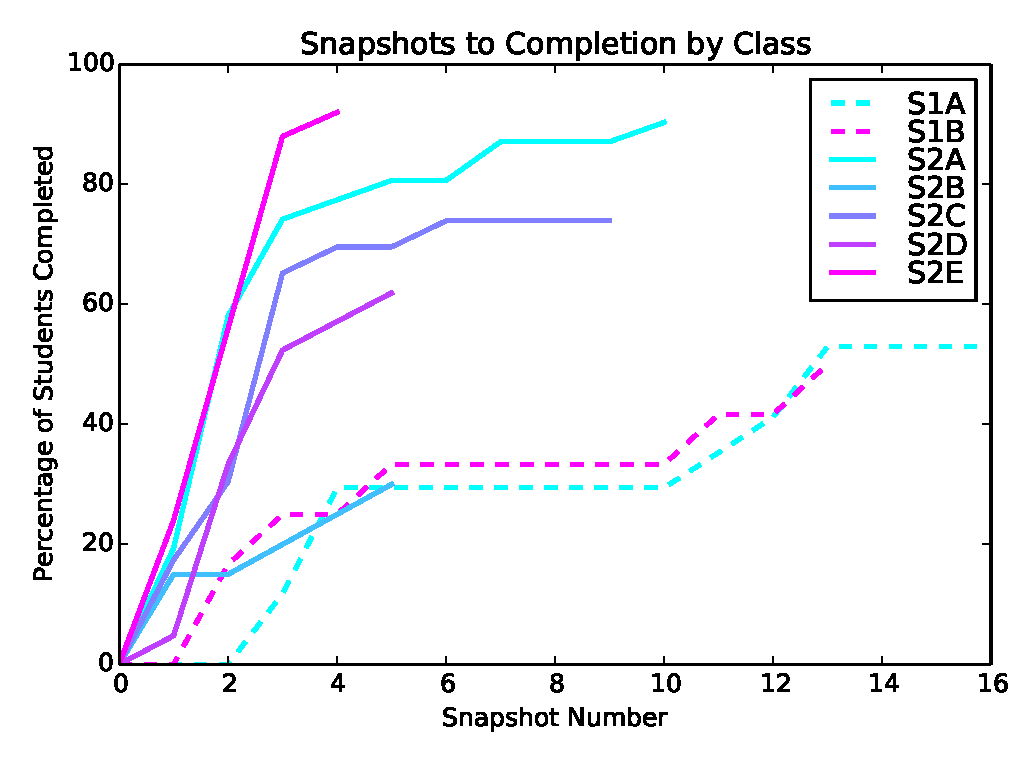
\includegraphics[width=5.25in]{graphs/snapshots_to_completion.eps}
\caption{Depicts the percentage of students by class that completed the
  assignment by the number of snapshots indicated on the x-axis. The dashed
  cyan line representing \emph{S1A} was truncated. It would otherwise extend
  horizontally out to the twenty-first snapshot.}
\locallabel{fig:snapshots_to_completion}
\end{figure}

In the previous section we looked at the total number of sprites \caught{} by
students in the seven classes analyzed. While this information provides us with
the overall completion rate, it does not provide any insight related to the
difficulty of the assignment. We approximate the assignment difficulty for a
student as the number of snapshots saved up to their first \com{}
snapshot. Recall from Section~\localref{sub:collection} that we consider each
snapshot to be a unit of work.

Figure~\localref{fig:snapshots_to_completion} plots the number of snapshots
saved for students in each class on their path to completion. An increase in
the \emph{y-value} for a line indicates what percent more students were able to
\com{} the assignment after the corresponding number of snapshots. The end of a
line indicates the maximum number of snapshots generated on the path to
completion for students of that class. This figure clearly conveys two
discrepancies between \sone{}, indicated by dashed-lines, and \stwo{},
indicated by solid-lines:

\begin{itemize}
\item All \stwo{} classes, save for \emph{S2B}, had a higher completion rate
  than the two \sone{} classes.
\item More importantly, this figure shows that \stwo{} was considerably less
  difficult to complete than \sone{} based on the strictly fewer number of
  snapshots to completion for all \stwo{} classes, again save for \emph{S2B}.
\end{itemize}

Over 50\% of \stwo{} students completed by snapshot three, whereas fewer than
25\% of \sone{} students completed by their third snapshot. Furthermore,
approximately 20\% of \sone{} \com{} students required more than ten snapshots
to complete the assignment. \stwo{} was less challenging to the students due in
part to the addition of the \glideto{} block. We look specifically at the
impact of the \glideto{} block in the next section.

\subsection{Approach to Solving the Assignment}
\locallabel{sub:approach}
As previously described, this assignment asks students to program a set of
directions to navigate the \net{} to \catch{} the \bear{}, the \horse{},
and the \zebra{}. This set of directions can be constructed in a number of
ways. At the highest level, there are two approaches:

\textbf{Glide to SPRITE}: With a single \glideto{} block the \net{} will glide
on a direct path to the target sprite resulting in an intersection between
two. The simplest \com{} solution requires only three of these blocks, one for
each of the \bear{}, the \horse{}, and the \zebra{}. This approach was only
available in \stwo{}.

\textbf{Orient and Glide}: The other high-level approach is to modify the
\net{'s} orientation via one of three classes of orientation changing blocks,
and then to glide an appropriate number of steps via a \glideDIST{} block in
order to reach the desired target or waypoint. The three classes of orientation
changing blocks are:

\textbf{Absolute orientation}: This orientation change is accomplished via a
\pointDIR{} block where \emph{X} can be selected as \emph{up (0)}, \emph{right
  (90)}, \emph{down (180)}, or \emph{left (-90)}. Alternatively, any number can
be manually entered for a more precise orientation. These orientations are
absolute with respect to the \stage{} meaning \emph{up} always orients toward
the top of the \stage{}, \emph{right}, toward the right of the \stage{}, etc.

\textbf{Relative orientation}: This orientation change is accomplished via
either a \emph{turn clockwise NUM degrees}, or a \emph{turn counterclockwise
  NUM degrees} block. The use of one of these blocks results in a modification
to the current orientation of the \net{}. That is, if the \net{} is oriented
toward the right of the \stage{}, a \emph{turn clockwise 90 degrees} block will
result in the \net{} being oriented toward the bottom of the \stage{}; in this
particular case, the \abs{} orientation block \pointDIR[down]{} would have the
same effect.

\textbf{Sprite orientation}: The third type of orientation change is
accomplished via a \pointtoward{} block. When invoked as
\pointtoward[\zebra{}]{}, the \net{} will orient itself toward the
\zebra{}. This block was only made available in \stwo{}.

A student may utilize a combination of these high-level approaches to complete
the assignment. For instance, in a single snapshot a student may use the
\emph{orient and glide} approach via a \rel{} orientation block to \catch{} the
\bear{}, and subsequently use the \glideto{} approach to \catch{} the
\horse{}. Alternatively, students may utilize several different classes of
orientation blocks. We wanted to see which combination of approaches was most
preferred among students who completed the assignment.

As mentioned in Section~\localref{sub:s1}, the base-project used as the
starting point for all students utilized an \abs{} orientation approach. In
order to accurately assess what approach combination the students explicitly
utilized, the code provided in the base-project was excluded from our approach
combination analysis.

\begin{figure}[!t]
\centering
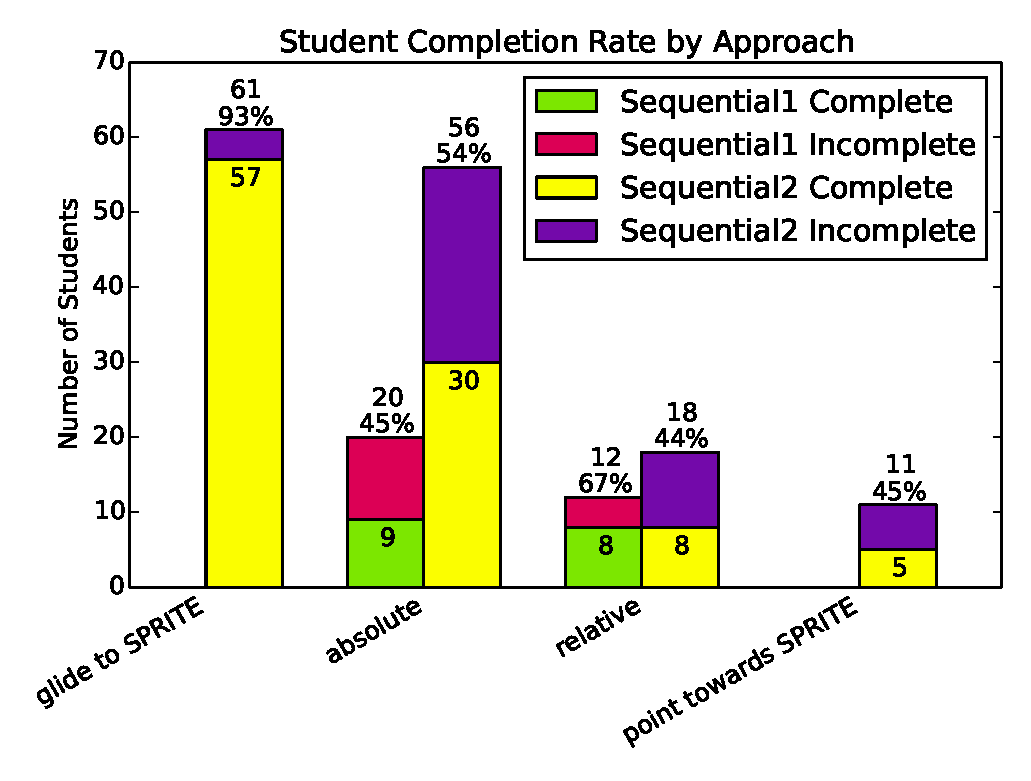
\includegraphics[width=5.25in]{graphs/approach_student_success.eps}
\caption{Shows the completion rate of each approach by student grouped by
  \sone{} and \stwo{}. An approach for a student is \com{} if any of the
  student's \com{} snapshots utilizes that approach. An approach for a student
  is \incom{} if they utilize the approach in any \incom{} snapshot and the
  approach is not found in any of the student's \com{} snapshots.}
\locallabel{fig:approach_student_success}
\end{figure}

Figure~\localref{fig:approach_student_success} shows a comparison of the
overall completion rate by student of each approach by assignment
iteration. Only snapshots up to a student's first \com{} snapshot are included
in this analysis as some teachers provided additional challenges to students
who had completed the assignment. The height of each bar indicates the total
number of students who had at least one snapshot that utilized the indicated
approach. This value is provided as the upper-most number above the bar. The
lower number is the completion rate as a percentage, and the number within the
lower segment of the bar quantifies the number of \com{} students for the
approach. An approach is \com{} for a student if they utilized that approach in
their first \com{} snapshot, otherwise, an approach is \incom{} for a
student. An approach is counted even when used in combination with another
approach. When comparing the fifteen \sone{} \com{} students to the
eighty-seven \stwo{} \com{} students, only two and fifteen respective \com{}
students (13.3\% and 17.2\%) utilized a combination of approaches in their
first \com{} snapshot.

This figure shows overwhelming evidence that students understood how to use
\glideto{} as the approach was \com{} for all but four (93.4\%) students who
attempted the approach. Conceptually, this observation makes sense as the
approach requires only a single block per \catch{}, rather than two or more
blocks as required by other approaches.

The \abs{} approach had around a 50\% completion rate for both \sone{} and
\stwo{}. Considering that all students were provided with a base-project
utilizing the \abs{} approach to \catch{} the \zebra{}, this result indicates
students struggled with the \abs{} approach.

While there are not many students for \sone{}, the figure does not convey that
all of the \com{} snapshots for the \rel{} approach belong to students in the
\emph{S1A} class. In fact, only one \emph{S1B} student attempted a \rel{}
approach, whereas all but four (76.5\%) \emph{S1A} students attempted an \abs{}
approach. None of our field notes provide any insight as to why the \rel{}
approach was so prominent with the \emph{S1A} class, especially when compared
to the insignificance of the \rel{} approach with \stwo{}.

Finally, we look at students' usage of an approach across snapshots in three
categories:

\begin{description}
\item[all] the student utilized the approach in at least one snapshot,
  including snapshots made following a \com{} snapshot
\item[up to last] the student utilized the approach in at least one snapshot up
  to and including their first \com{} snapshot (includes all snapshots for
  students who had no \com{} snapshot)
\item[last] the student utilized the approach in either their first \com{}
  snapshot, or their last snapshot if all of their snapshots were \incom{}
\end{description}

\begin{figure}[!t]
\centering 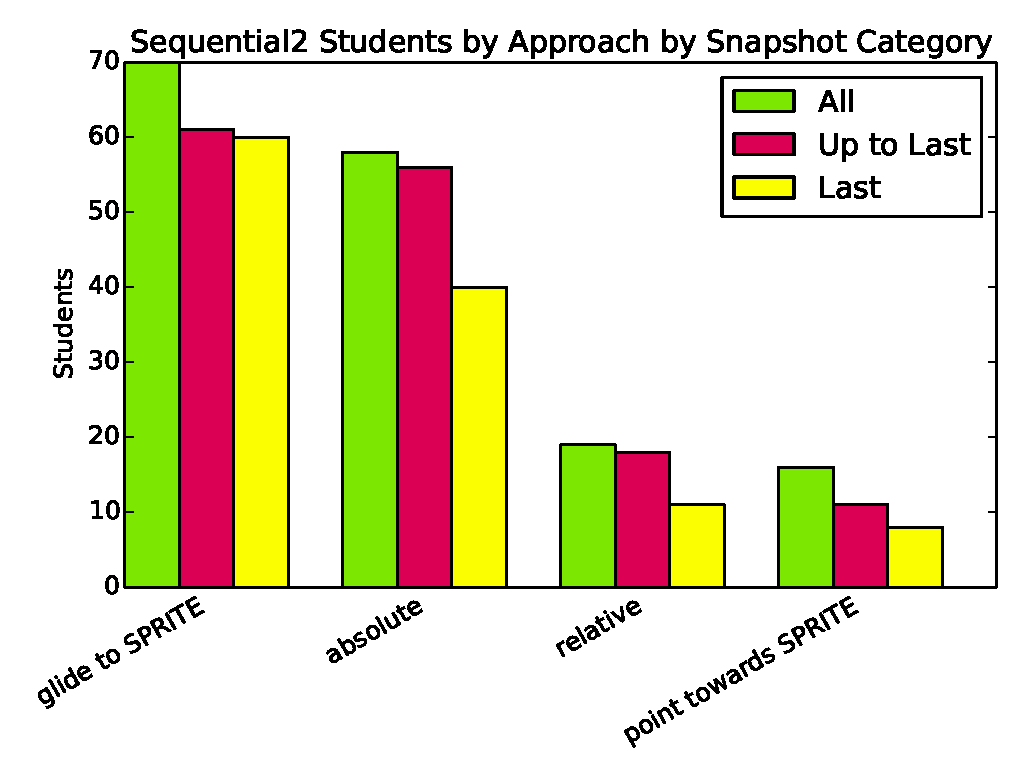
\includegraphics[width=5.25in]{graphs/approach_bar_Sequential2.eps}
\caption{Shows how many students utilized each approach in \stwo{} snapshots
  for three categories: \emph{all} snapshots, snapshots up to the first \com{}
  or last \incom{}, and the \emph{last} snapshot.}
\locallabel{fig:approach_bar_s2}
\end{figure}

Figure~\localref{fig:approach_bar_s2} quantifies the number of students who
utilize each approach in \stwo{} snapshots for each of the aforementioned
categories. There are two primary observations: The first is that the
difference in height between the pink and yellow bars show the number of
students who abandoned an approach. The minuscule difference for the \glideto{}
approach provides additional evidence for the ease-of-use of that approach. We
make no claims about the abandonment of other approaches due to the low number
of students utilizing those approaches. The second observation pertains to the
difference in height between the pink and green bars for each category. This
difference indicates students who, only after making their first \com{}
snapshot, attempted a new approach. These additional attempts made by students
after a \com{} snapshot are likely due to additional challenges posed by
instructors. The figure shows very little growth in the \abs{} and \rel{}
approaches, but a nearly 15\% increase in the \glideto{} approach; once again
providing support for the ease-of-use of the \glideto{} approach. A figure for
\sone{} is not provided as there are only two possible approaches, and none of
the students switched approaches after their first \com{} snapshot.

\subsection{Quantifying Students Affected by a Scratch Race Condition}
\locallabel{sub:race}

Our curriculum development and testing process, as described in
Section~\localref{sec:methodology} and visualized in
Figure~\localref{fig:process}, allowed us to focus analysis on issues we became
aware of due to the in-class researchers' field notes. However, the field notes
did not always capture the relevant information. During manual analysis of the
students' snapshots we noticed a number of snapshots that produced inconsistent
results across multiple executions. These snapshots should have consistently
\caught{} the \zebra{}, however, only did so approximately 50\% of the time. We
discovered the problem to be a race condition within Scratch where the
detection of the intersection between two sprites may not occur in the brief
period of time that the sprites intersect. Instead, the next block in the
script, always a rotation block, would execute and the rotation would result in
the separation of the two sprites; i.e., the two sprites were no longer
intersecting. In-class education researchers confirmed having observed this
issue, however, their field notes did not quantify the number of students
affected. We hypothesized that students affected by this issue may have
struggled completing the assignment.

In order to quantify the students affected, we wrote a Hairball plugin to track
the \net{'s} \exe{}, i.e., the sequence of blocks beginning with
\netclicked{}. We wanted to discover snapshots where the \net{'s} \exe{}
matches that of one of the \exe{s} we manually verified as exhibiting the race
condition. We manually verified \exe{s} by programming them in Scratch, and
executing the \sprogram{} up to twenty times. If we observed inconsistency in
the \catch{ing} of the \zebra{} within these twenty executions, then the \exe{}
was labeled as exhibiting the race condition; otherwise it was not. While it is
possible for a race condition to emerge at a lessor frequency, we assume that
few, if any, students were affected by these cases. No race condition
exhibiting \exe{} required more than eight executions to detect.

What resulted was a Hairball plugin with a state machine that handled all
\exe{s} of the \net{} shared by more than any ten snapshots. We only handled
\exe{s} up to the point that we could label them as exhibiting the race
condition or not. Of the 297 and 638 snapshots for \sone{} and \stwo{}
respectively, only thirty-nine and thirty-eight respective snapshots (13\% and
6\%) contained an \exe{} not explicitly handled by our plugin.

In addition to labeling \exe{s} exhibiting the race condition, we labeled those
resulting in a consistent intersection with the \zebra{}. Students with such a
snapshot subsequent to a snapshot exhibiting the race condition are likely to
have expended effort to resolve the race condition. We label these snapshots as
\emph{fixed}. Additionally, for each student with one or more snapshots
exhibiting the race condition, we consider whether or not they completed the
assignment.

\begin{figure}[!t]
\centering 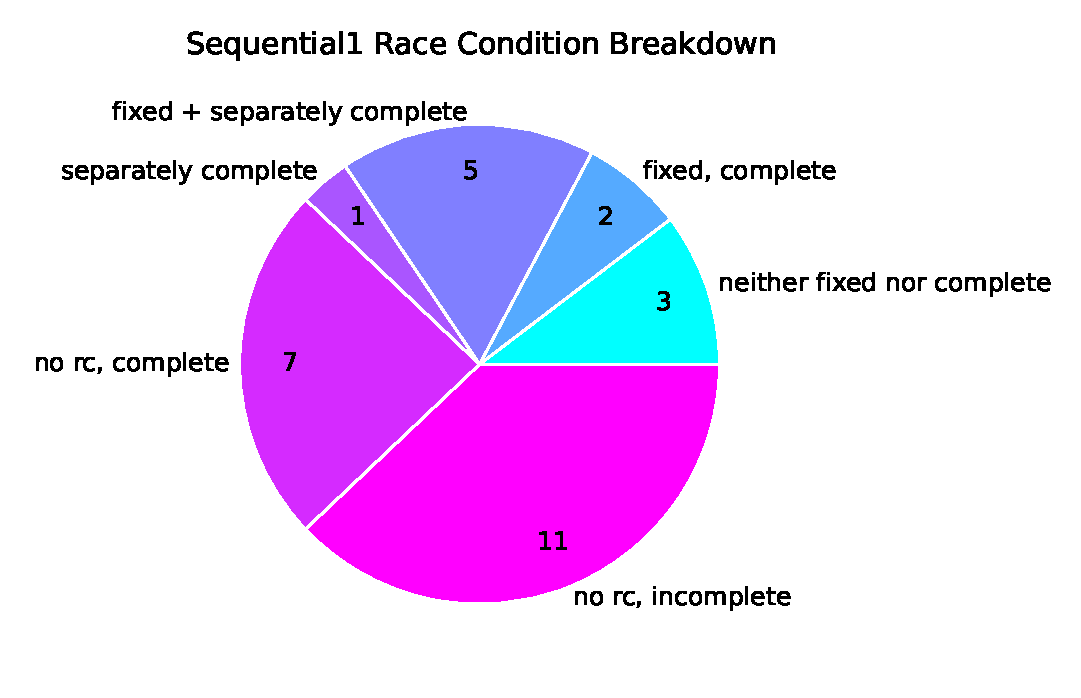
\includegraphics[trim=0 .48in 0 0, clip, width=5.45in]{graphs/race_condition_Sequential1.eps}
\caption{Shows the breakdown of students affected by the race condition issue
  in Scratch for \sone{}.}
\locallabel{fig:rc_s1}
\end{figure}

\begin{figure}[!t]
\centering 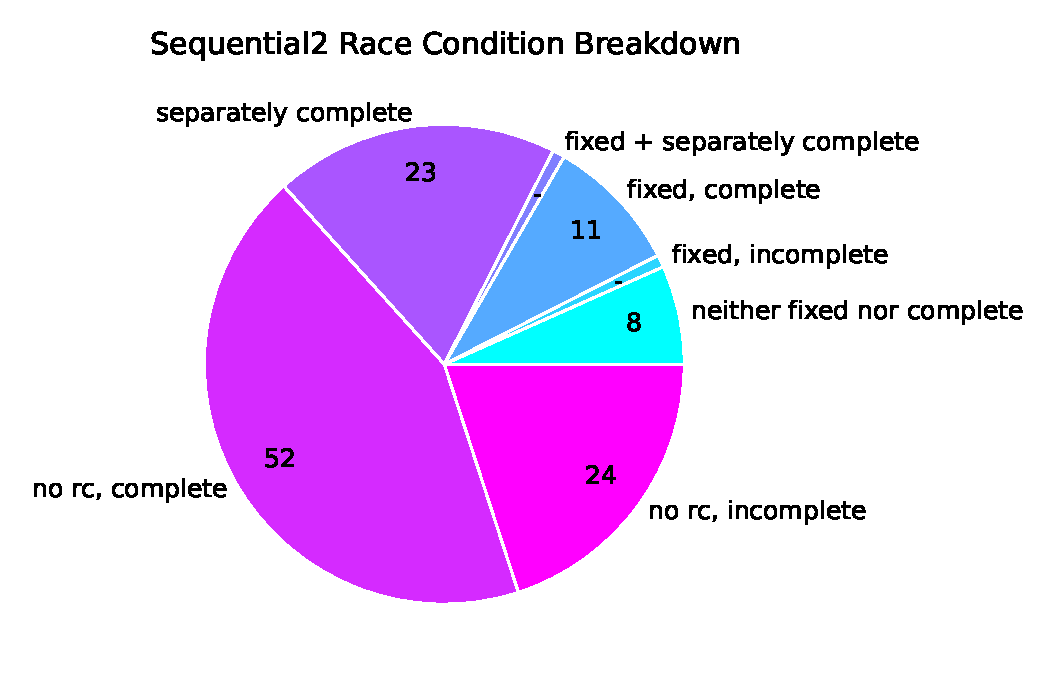
\includegraphics[trim=0 .5in 0 0, clip, width=5.30in]{graphs/race_condition_Sequential2.eps}
\caption{Shows the breakdown of students affected by the race condition issue
  in Scratch for \stwo{}.}
\locallabel{fig:rc_s2}
\end{figure}

Figure~\localref{fig:rc_s1} and Figure~\localref{fig:rc_s2} show the breakdown
of all students grouped by whether or not they have at least one snapshot
exhibiting the race condition. In total eleven and forty-four students (38\%
and 37\%) have snapshots exhibiting the race condition for \sone{} and \stwo{}
respectively. Of those, three and nine students (27\% and 20\%) were unable to
complete the assignment. Six and twenty-four students (55\% and 55\%) took a
completely separate approach to completing the assignment after experiencing
the race condition, whereas only two and eleven students (18\% and 25\%) solved
the assignment by the addition of one or more blocks that \emph{fixed} the race
condition.

Fortunately, a majority of students were able to avoid the race condition. We
sampled the snapshots of a few of these students and discovered the following
three approaches that students used to avoid encountering the race condition:

\begin{enumerate}
\item The student immediately removed some or all of the provided code thus
  starting with a modified base-project.
\item In \stwo{}, the student simply appended \glideto{} blocks to the code.
\item The student immediately added an additional \glideDIST{} block resulting
  in consistent intersection between the \net{} and the \zebra{}.
\end{enumerate}

Students were also able to \emph{fix} the race condition using the above
approaches. Of the thirteen students who first encountered, and then resolved
the race condition, two students (15.4\%) \emph{fixed} the race condition using
approach~\#2, and the remaining eleven students (84.6\%) \emph{fixed} using
approach~\#3. Note that while students may have used the same approach to avoid
the race condition, only students for whom we have a prior snapshot exhibiting
the race condition are labeled as \emph{fixed} in Figure~\localref{fig:rc_s1}
and Figure~\localref{fig:rc_s2}.

The data show that over one third of students experienced the race
condition. Interestingly, the students who experienced the race condition were
statistically significantly more likely to complete the assignment: 73\% and
82\% compared to 39\% and 68\% (chi square, p \textless{} 0.028). This result
was unexpected, nevertheless, the labels provided by our static analysis
indirectly allowed us to discover the primary reason why students who did not
experience the race condition, did not complete the assignment. Manual
inspection of these labeled snapshots revealed that a large majority of these
students either removed, or significantly altered the provided code in their
first snapshot. The only other reason we discovered was due to race condition
avoidance approach~\#3 where, in each of these cases, it was apparent that the
avoidance of the race condition was unintentional based on the subsequent
erratic modifications made by these students.

Overall, the effect of these results is that we are now able to adjust our
assignment so that students are less likely to encounter a Scratch race
condition. Moreover, given the negative impact of students removing the
provided code, we learned that preventing students from doing so may have a
positive effect on learning.

\subsection{Snapshots Exhibiting the \emph{Double Click to Execute} Behavior}
\locallabel{sub:dce}

Scratch is built such that students can double click on any script, i.e., one
or more connected blocks, in order to execute that script. During \sone{},
in-class education researchers described in their field notes that some
students took advantage of this behavior in order to execute scripts they
created. While manually executing disjoint scripts in this manner may trigger
the success screen we built into the assignment, the education researchers
found that students exhibiting this behavior did not understand the concept of
a script. Instead, these students viewed the blocks as independent entities not
sequentially triggered by an event (e.g., \netclicked{}), and therefore these
students did not exhibit the conceptual understanding of sequential execution
we had intended. Furthermore, the education researchers noted that students
would \dce{} a script in order to move from the start location to the first
sprite, and then alter that script to perform the next step of the
sequence. Thus, as another use of scaffolding in the assignment, we disabled
the \dce{} feature in \stwo{} in attempt to prevent students from going down an
unintended path while completing the assignment.

\subsubsection{Double Click to Execute Filters}
Once aware of the problem, we sought to retroactively identify students who may
have utilized this \dce{} approach. Ideally, we wanted a plugin that would
positively identify these students based on their snapshots. However, with the
information provided in the snapshots we could only incrementally filter out
snapshots matching models that we verified do not demonstrate the \dce{}
behavior. The following paragraphs detail, in order, the static analysis
filters we created in attempt to approximate the students affected by the
\dce{} behavior.

\begin{description}
\item [\emph{Complete} Snapshots] Any snapshots that when emulated by our
  plugin result in the \net{} \catch{ing} any two or more sprites are
  filtered. Furthermore, any chronologically subsequent snapshots by the same
  student are filtered. The subsequent snapshots are filtered because, once a
  student demonstrates success, we are not concerned about their \dce{} use.
\item [Motionless Snapshots] Any snapshots that result in no movement due to
  either having zero scripts or having only a single \netclicked{} script with
  no movement blocks are filtered. These snapshots do not result in any motion
  and thus are not indicative of \dce{} behavior that we are concerned with.
\item [\net{} Ends in Expected Location] Each \sprogram{}, i.e., each snapshot,
  stores the last location of all its sprites. We compare the stored location
  of the \net{} to its final location as computed by our \net{} emulation
  Hairball plugin. Snapshots containing movement whose emulated \net{} location
  matches the \net{'s} stored location are filtered. These snapshots are
  filtered because our emulation plugin does not support the \dce{} behavior,
  thus it is not possible for these locations to match when the \dce{} behavior
  is used.
\item [Multiple \net{} Clicks] We expect students' scripts to execute only once
  upon \netclicked{} following a reset of the environment via a click on the
  \emph{green flag}. However, it is still possible to click on the \net{}
  multiple times resulting in an execution for each of these clicks. In such
  cases, the \net{} will initially be in an invalid state for all but the first
  \net{} click. By performing the expected location test multiple times we are
  able to both identify and filter snapshots exhibiting this multiple \net{}
  click behavior. These snapshots are filtered for the same reason as those
  filtered due to ending in an expected location.
\end{description}


\subsubsection{Double Click to Execute Snapshots}

\begin{figure}[!t]
\centering 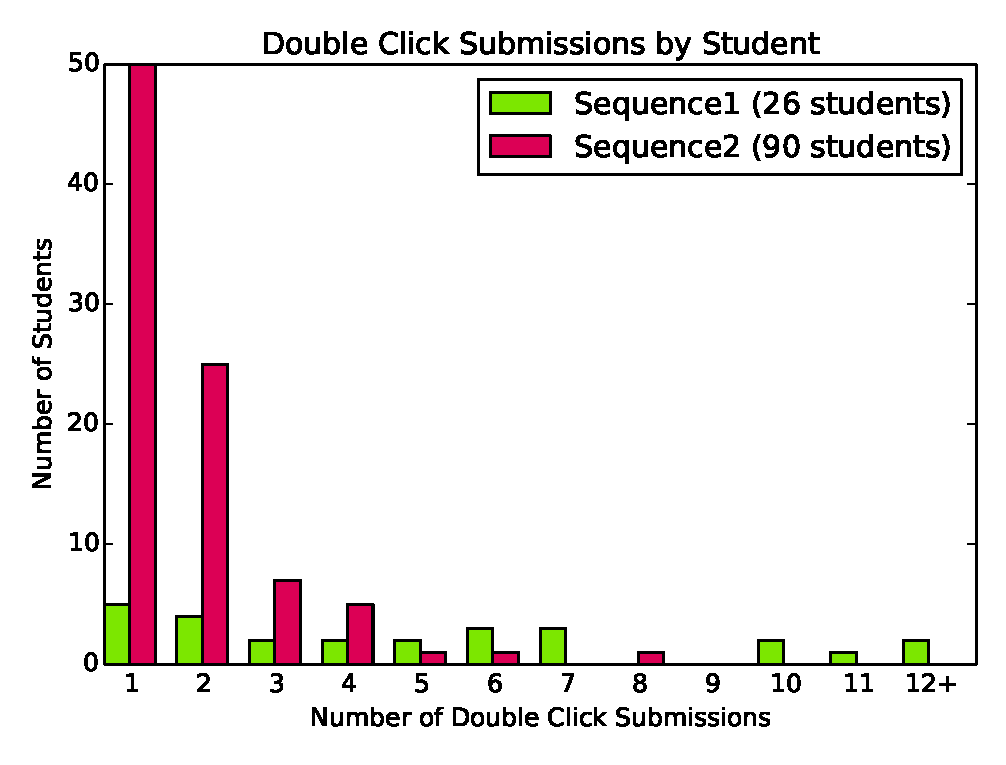
\includegraphics[width=5.25in]{graphs/dc_submissions.eps}
\caption{Depicts the number of \dce{} snapshots we identified for each
  student.}
\locallabel{fig:dc_snapshots}
\end{figure}

After applying all the filters, we counted the number of remaining snapshots
per student that may exhibit the \dce{}
behavior. Figure~\localref{fig:dc_snapshots} shows the number of potential
snapshots by student for both \sone{} and \stwo{}. Recall that the \dce{}
functionality was disabled completely in \stwo{}, thus we hoped that this
filtering would result in nearly zero \stwo{} snapshots and a significant
decrease in the number of \sone{} students whose snapshots we would manually
inspect. However, that was not the case. In reality, this filtering only
removed three of twenty-nine and thirty of 120 students (10.3\% and 25.0\%)
respectively. Unfortunately, without more precise field notes, we cannot
quantify the number of students affected because there is not sufficient
information in the snapshots for us to even manually identify students
exhibiting the \dce{} behavior.

It is important to note that while we could not proceed, it was not due to a
limitation of static analysis. The Hairball plugin we wrote considerably helped
us come to the conclusion that we simply had not gathered enough information to
either manually or automatically determine the students affected by the \dce{}
behavior. Based on this experience with a lack of data, we are altering our
data collection to capture every change made by students.
